\section{(Somewhat) Practical Anonymous Routing}
The main protocol.

\subsection{Server Write}

%%%
%%% Server combine
%%%
\begin{algorithm}
\caption{Homomorphic placing $\mathsf{HomPlacing}$}
\label{alg:spar:write}
\begin{algorithmic}[1]
    % \Require An encrypted value $V_r$ and $\log{n}$ bits $\{c_0,\dots,c_{L-1}\}$, where $L = \log{n}$
    % \Ensure A vector $\mathbf{l}$ consisting of $n$ values of leaves: $z_0, \dots, z_{n-1}$, where $\mathbf{l}[i] = z_i$ for $i \in \{0,\dots, n-1\}$
    
    \State let $\mathsf{notHasWritten = \mathsf{RGSW}^*(1)}$
    \For{$d \leftarrow \{0,1,2\}$}
        \For{$k \leftarrow \{0,1,2\}$}
            \For{$i \leftarrow \{0, \dots, \eta - 1\}$}
                \State let $h = z_{i,d}\boxtimes I_{i,k} \boxtimes \mathsf{notHasWritten}$
                \State $L_{i,k} := L_{i,k} + h\cdot V_r$
                \State $I_{i,k} := I_{i,k} - h$
                \State $\mathsf{notHasWritten} := \mathsf{notHasWritten} - h$
            \EndFor
        \EndFor
    \EndFor
    \State\Return $\mathsf{notHasWritten}$
\end{algorithmic}
\end{algorithm}

$^*$ The server has no obligation to encrypt its values ($\mathsf{notHasWritten}, L, I$) and may in some cases even be actively trying to break privacy and thus cannot be trusted to add any noise. This improves the performance of the algorithm as noiseless ``encryption'' is marginally faster as it does not need to perform any random sampling, and makes the algorithm as a whole more tolerable to noise.

\ifnotes
\begin{itemize}
    \item Big challenge $\to$ Implement RGSW ciphertext for BFV/BGV
    \begin{itemize}
        \item External product implementation; should be easy to implement once RGSW ciphertext is implemented
    \end{itemize}
\end{itemize}
\fi

\subsection{HomPlacing}
Algorithm 1 shows the idea of Algorithm 2.

\begin{itemize}
    \item From \gls{niar}: sorting of random numbers = shuffling.
    \item Evaluate tree, each bit determines if the data is placed left or right. One level per bit means there are $2^n$ buckets in the end, each one representing a bit string i.e. 000, 001, 010, 011, 100, 101, 110, 111 for 3 bits.
    \item We can encode the bits into \gls{rgsw} form.
\end{itemize}

\begin{figure}[ht!]
    \centering
    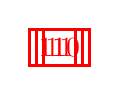
\begin{tikzpicture}[
    level 1/.style={sibling distance=0cm},
    level 2/.style={sibling distance=0.25cm},
    level 3/.style={sibling distance=1.45cm},
    level distance=2cm,
    % Define a reusable style for highlighted edges
    highlight/.style={draw=red, text=red, very thick}
]
\Tree [.ciphertext
  \edge node[auto=right]{0};              % label the left edge "0"
  [.0
    \edge node[auto=right]{0};
    [.00
      \edge node[auto=right]{0};  [.000 ]
      \edge node[auto=left]{1}; [.001 ]
    ]
    \edge node[auto=left]{1};
    [.01
      \edge node[auto=right]{0};  [.010 ]
      \edge node[auto=left]{1}; [.011 ]
    ]
  ]
  \edge[highlight] node[auto=left]{1};             % label the right edge "1"
  [.\node[highlight]{1};
    \edge node[auto=right]{0};
    [.10
      \edge node[auto=right]{0};  [.100 ]
      \edge node[auto=left]{1}; [.101 ]
    ]
    \edge[highlight] node[auto=left]{1};
    [.\node[highlight]{11};
      \edge[highlight] node[auto=right]{0}; [.\node[highlight]{110}; ]
      \edge node[auto=left]{1}; [.111 ]
    ]
  ]
]
\end{tikzpicture}
    \caption{HomPlacing tree with a 3-bit index $a$. At level $i$, the $i$-th MSB of the index $a$ determines homomorphically wether the ciphertext is placed in the left (0) or right (1) bucket. This process is repeated $\log{n}=3$ times until the ciphertext is placed in the $a$-th bucket, without the placer ever knowing which bucket that is. The highlighted path shows the route taken for the index $a = 6 = [110]_2$: the MSB places the ciphertext in the right bucket, and so on. Again, the server doesn't know $a$, only the \emph{encryption} of the bits $[a]_2$. % \textcolor{red}{MSB or LSB, what direction is used originally?}
    }
    \label{fig:hom-placing-1}
\end{figure}

\input{Algorithms/spar-1}
\clearpage

% % TODO: Place in pre-amble
% \definecolor{codebg}{rgb}{0.25, 0.25, 0.25}
% \setminted{bgcolor=codebg}
% \usemintedstyle{native}

% \begin{listing}[!ht]
% \inputminted{cpp}{Code/spar-1.hpp}
% \caption{Algorithm 1 from sPAR implemented in C++ with OpenFHE}
% \label{listing:sPAR:Algorithm-1}
% \end{listing}